\section{Derivadas Parciales}

El análisis de funciones de varias variables requiere una noción de tasa de cambio que respete la estructura multidimensional del dominio. En una variable, la derivada mide cómo cambia $f(x)$ cuando $x$ varía. En varias variables, la pregunta más natural es: ¿cómo cambia $f(x, y)$ cuando solo una de las variables varía, mientras la otra permanece fija? La respuesta a esta pregunta es la derivada parcial.

\subsection{Definición}

\begin{mydefinition}{Derivada parcial}
Sea $f: D \subseteq \mathbb{R}^2 \to \mathbb{R}$ y sea $(x_0, y_0)$ un punto interior del dominio $D$. La derivada parcial de $f$ con respecto a $x$ en $(x_0, y_0)$ se define como:
\[
\frac{\partial f}{\partial x}(x_0, y_0) = \lim_{h \to 0} \frac{f(x_0 + h,\, y_0) - f(x_0,\, y_0)}{h}
\]
siempre que el límite exista. De forma análoga, la derivada parcial con respecto a $y$ en $(x_0, y_0)$ es:
\[
\frac{\partial f}{\partial y}(x_0, y_0) = \lim_{h \to 0} \frac{f(x_0,\, y_0 + h) - f(x_0,\, y_0)}{h}
\]
\end{mydefinition}

La estructura de la definición es idéntica a la de la derivada ordinaria: se perturba una sola variable, se mide el cociente de diferencias y se toma el límite. La única diferencia es que la otra variable permanece constante durante el proceso.

\textbf{Ejemplo.} Sea $f(x, y) = x^2 + xy$. Por definición:
\[
\frac{\partial f}{\partial x}(1, 2) = \lim_{h \to 0} \frac{(1+h)^2 + (1+h) \cdot 2 - (1 + 2)}{h}
= \lim_{h \to 0} \frac{h^2 + 2h + 2h}{h} = \lim_{h \to 0} (h + 4) = 4
\]

\subsection{Notaciones}

Para una función $z = f(x, y)$, la derivada parcial con respecto a $x$ admite varias escrituras equivalentes:
\[
\frac{\partial f}{\partial x} = \frac{\partial z}{\partial x} = f_x = \partial_x f = D_x f
\]
y de forma análoga para $y$:
\[
\frac{\partial f}{\partial y} = \frac{\partial z}{\partial y} = f_y = \partial_y f = D_y f
\]

Para indicar que la derivada se evalúa en un punto específico $(x_0, y_0)$ se escribe $f_x(x_0, y_0)$ o $\left.\dfrac{\partial f}{\partial x}\right|_{(x_0,y_0)}$.

La notación $f_x$ es compacta y útil en cálculos. La notación de Leibniz $\dfrac{\partial f}{\partial x}$ es más explícita y facilita la identificación de la variable de derivación, lo que la hace conveniente en contextos donde intervienen muchas variables.

\subsection{Cálculo de derivadas parciales}

\begin{mynote}{Regla práctica}
Para calcular $\dfrac{\partial f}{\partial x}$, se trata $y$ como una constante y se deriva con respecto a $x$ usando las reglas ordinarias de derivación. Para calcular $\dfrac{\partial f}{\partial y}$, se trata $x$ como una constante y se deriva con respecto a $y$.
\end{mynote}

Todas las reglas de derivación de una variable se aplican sin modificación: la regla del producto, la del cociente y la de la cadena funcionan igual, porque en cada derivada parcial solo hay una variable activa.

\textbf{Ejemplo 1.} Sea $f(x, y) = x^3 y^2 + 2xy - y^4$.
\[
f_x = 3x^2 y^2 + 2y \qquad f_y = 2x^3 y + 2x - 4y^3
\]

\textbf{Ejemplo 2.} Sea $g(x, y) = \sin(x^2 + y)$. Aplicando la regla de la cadena:
\[
g_x = \cos(x^2 + y) \cdot 2x \qquad g_y = \cos(x^2 + y)
\]

\textbf{Ejemplo 3.} Sea $h(x, y) = e^{xy} \ln y$. Al derivar con respecto a $x$ se trata $\ln y$ como constante, y al derivar con respecto a $y$ se aplica la regla del producto:
\[
h_x = y e^{xy} \ln y \qquad h_y = x e^{xy} \ln y + \frac{e^{xy}}{y}
\]

\subsection{Interpretación geométrica y conceptual}

Considérese la superficie $z = f(x, y)$ y un punto $(x_0, y_0, f(x_0, y_0))$ sobre ella. Si se intersecta la superficie con el plano vertical $y = y_0$, se obtiene una curva plana que puede verse como la gráfica de la función de una variable $z = f(x, y_0)$. La derivada parcial $f_x(x_0, y_0)$ es la pendiente de la recta tangente a esa curva en el punto considerado.

De forma análoga, la intersección con el plano $x = x_0$ da la curva $z = f(x_0, y)$, y $f_y(x_0, y_0)$ es la pendiente de su recta tangente.

\begin{center}
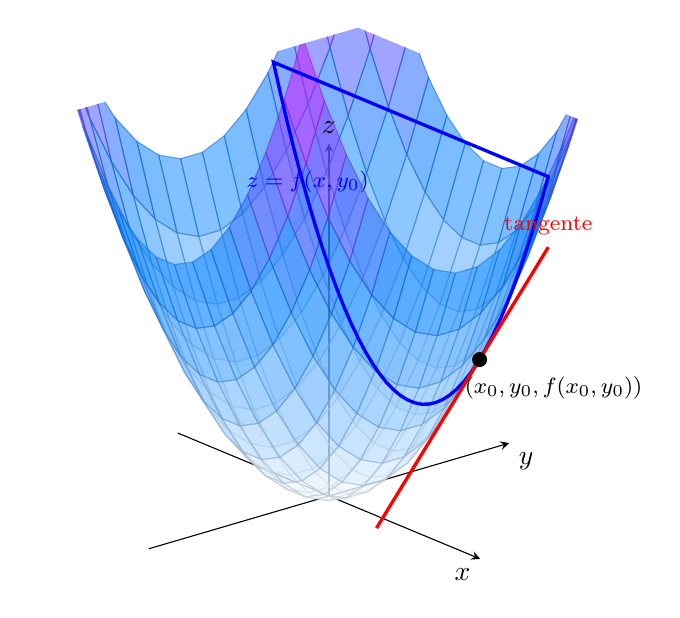
\begin{tikzpicture}
\begin{axis}[
    view={50}{25},
    axis lines=center,
    xlabel={$x$}, ylabel={$y$}, zlabel={$z$},
    xlabel style={anchor=north east},
    ylabel style={anchor=north west},
    zlabel style={anchor=south},
    xmin=-2.2, xmax=2.2,
    ymin=-2.2, ymax=2.2,
    zmin=0,    zmax=5,
    xtick=\empty, ytick=\empty, ztick=\empty,
    width=10cm, height=9cm,
    colormap/cool,
]
    % Superficie
    \addplot3[
        surf, opacity=0.55,
        domain=-2:2, domain y=-2:2,
        samples=16,
    ] {x^2 + y^2};

    % Curva de corte con y=1 (plano y=1)
    \addplot3[
        very thick, blue,
        domain=-2:2, samples=40,
    ] ({x}, {1}, {x^2 + 1});

    % Recta tangente en (1,1,2) con pendiente f_x=2x=2
    \addplot3[
        very thick, red,
        domain=-0.5:2.0, samples=2,
    ] ({x}, {1}, {2*(x-1) + 2});

    % Punto de tangencia
    \addplot3[mark=*, mark size=2.5pt, black] coordinates {(1,1,2)};

    \node[font=\footnotesize, blue] at (axis cs:-1.5, 1, 3.5) {$z = f(x,y_0)$};
    \node[font=\footnotesize, red]  at (axis cs: 2.0, 1, 4.3) {tangente};
    \node[font=\footnotesize, black, anchor=north west] at (axis cs:1,0.7,2)
        {$(x_0,y_0,f(x_0,y_0))$};
\end{axis}
\end{tikzpicture}
\end{center}

Conceptualmente, $f_x(x_0, y_0)$ mide la tasa de cambio instantánea de $f$ en la dirección del eje $x$ al pasar por $(x_0, y_0)$. Si $f_x > 0$, la función crece al moverse en esa dirección; si $f_x < 0$, decrece. La misma idea se aplica a $f_y$ en la dirección $y$. Cada derivada parcial da información sobre el comportamiento de $f$ en una dirección coordenada, sin decir nada sobre las demás.

\subsection{Generalización para $n$ variables}

La definición se extiende sin dificultad a funciones de $n$ variables.

\begin{mydefinition}{Derivada parcial en $\mathbb{R}^n$}
Sea $f: D \subseteq \mathbb{R}^n \to \mathbb{R}$ y sea $\mathbf{x}_0 = (x_1, \dots, x_n) \in D$ un punto interior. La derivada parcial de $f$ con respecto a la $i$-ésima variable en $\mathbf{x}_0$ es:
\[
\frac{\partial f}{\partial x_i}(\mathbf{x}_0)
= \lim_{h \to 0}
  \frac{f(x_1, \dots,\, x_i + h,\, \dots, x_n) - f(\mathbf{x}_0)}{h}
\]
\end{mydefinition}

Para calcularla, se fijan todas las variables excepto $x_i$ y se aplican las reglas ordinarias de derivación. El resultado es una función que, en general, depende de todas las variables.

\textbf{Ejemplo.} Sea $f(x, y, z) = x^2 yz + e^{xz}$.
\[
\frac{\partial f}{\partial x} = 2xyz + ze^{xz}
\qquad
\frac{\partial f}{\partial y} = x^2 z
\qquad
\frac{\partial f}{\partial z} = x^2 y + xe^{xz}
\]

\subsection{Derivadas parciales de orden superior}

Si $f_x$ y $f_y$ son a su vez diferenciables, se pueden calcular sus derivadas parciales, obteniendo derivadas de segundo orden. Para $f(x, y)$ existen cuatro:

\[
f_{xx} = \frac{\partial^2 f}{\partial x^2}
       = \frac{\partial}{\partial x}\!\left(\frac{\partial f}{\partial x}\right)
\qquad
f_{yy} = \frac{\partial^2 f}{\partial y^2}
       = \frac{\partial}{\partial y}\!\left(\frac{\partial f}{\partial y}\right)
\]
\[
f_{xy} = \frac{\partial^2 f}{\partial y\,\partial x}
       = \frac{\partial}{\partial y}\!\left(\frac{\partial f}{\partial x}\right)
\qquad
f_{yx} = \frac{\partial^2 f}{\partial x\,\partial y}
       = \frac{\partial}{\partial x}\!\left(\frac{\partial f}{\partial y}\right)
\]

Las derivadas $f_{xx}$ y $f_{yy}$ se denominan derivadas puras, y $f_{xy}$, $f_{yx}$ se denominan derivadas mixtas. En la notación de Leibniz, el orden de derivación se lee de derecha a izquierda: $\dfrac{\partial^2 f}{\partial y\,\partial x}$ indica que se deriva primero con respecto a $x$ y luego con respecto a $y$.

El proceso se puede iterar para obtener derivadas de cualquier orden. Una derivada de orden $k$ se obtiene aplicando $k$ veces la operación de derivación parcial, posiblemente con respecto a variables distintas.

\textbf{Ejemplo.} Sea $f(x, y) = x^3 y + \sin(xy)$.
\[
f_x = 3x^2 y + y\cos(xy) \qquad f_y = x^3 + x\cos(xy)
\]
\[
f_{xx} = 6xy - y^2\sin(xy) \qquad f_{yy} = -x^2\sin(xy)
\]
\[
f_{xy} = 3x^2 + \cos(xy) - xy\sin(xy) \qquad f_{yx} = 3x^2 + \cos(xy) - xy\sin(xy)
\]

Se observa que $f_{xy} = f_{yx}$. Esta igualdad no es casual: es consecuencia del teorema de Clairaut.

\subsection{Teorema de Clairaut}

\begin{mytheorem}{Teorema de Clairaut}
Sea $f: D \subseteq \mathbb{R}^2 \to \mathbb{R}$. Si las derivadas mixtas $f_{xy}$ y $f_{yx}$ están definidas en un entorno abierto del punto $(x_0, y_0)$ y son continuas en $(x_0, y_0)$, entonces:
\[
f_{xy}(x_0, y_0) = f_{yx}(x_0, y_0)
\]
\end{mytheorem}

La hipótesis de continuidad es necesaria: existen funciones para las que $f_{xy}$ y $f_{yx}$ existen en un punto pero son distintas, precisamente porque alguna de las dos no es continua allí.

\textbf{Ejemplo de aplicación.} Sea $f(x, y) = e^{x^2 y}$. Se tiene:
\[
f_x = 2xy\, e^{x^2 y} \qquad f_{xy} = \frac{\partial}{\partial y}(2xy\, e^{x^2 y}) = 2x\, e^{x^2 y} + 2x \cdot x^2 y\, e^{x^2 y} = 2x(1 + x^2 y)\,e^{x^2 y}
\]
\[
f_y = x^2 e^{x^2 y} \qquad f_{yx} = \frac{\partial}{\partial x}(x^2 e^{x^2 y}) = 2x\,e^{x^2 y} + x^2 \cdot 2xy\,e^{x^2 y} = 2x(1 + x^2 y)\,e^{x^2 y}
\]
Como ambas derivadas son continuas, el teorema garantiza $f_{xy} = f_{yx}$, lo que se verifica directamente.

El teorema se extiende a funciones de $n$ variables y a derivadas mixtas de cualquier orden: si todas las derivadas parciales de orden $k$ son continuas, el resultado no depende del orden en que se apliquen las $k$ derivaciones.

\subsection{Ejercicios}

\begin{enumerate}
    \item Calcule $f_x$ y $f_y$ usando la definición de límite para cada función en el punto indicado.
\begin{enumerate}
    \item $f(x, y) = 3x^2 - 2xy$ en $(1, 1)$
    \item $f(x, y) = xy^2 + x$ en $(2, 1)$
\end{enumerate}

    \item Calcule todas las derivadas parciales de primer orden.
\begin{enumerate}
    \item $f(x, y) = x^4 - 3x^2y^3 + y^5$
    \item $g(x, y) = \dfrac{x^2 - y}{x + 2y}$
    \item $h(x, y) = \sqrt{x^2 + y^2 + 1}$
\end{enumerate}

    \item Calcule las derivadas parciales de primer orden de las siguientes funciones.
\begin{enumerate}
    \item $f(x, y) = e^{x^2 + y^2}$
    \item $g(x, y) = \ln\!\left(x^2 + \sin y\right)$
    \item $h(x, y) = \arctan\!\left(\dfrac{y}{x}\right)$
\end{enumerate}

    \item Calcule las derivadas parciales de primer orden de las siguientes funciones de tres variables.
\begin{enumerate}
    \item $f(x, y, z) = x^2 y - yz^3 + xz$
    \item $g(x, y, z) = e^{xyz}$
    \item $h(x, y, z) = \dfrac{x + y}{y + z}$
\end{enumerate}

    \item Calcule las cuatro derivadas parciales de segundo orden $f_{xx}$, $f_{yy}$, $f_{xy}$ y $f_{yx}$.
\begin{enumerate}
    \item $f(x, y) = x^3 y^2 - 5xy^4$
    \item $f(x, y) = \cos(x + 2y)$
    \item $f(x, y) = x \ln(xy)$
\end{enumerate}

    \item Verifique el teorema de Clairaut calculando $f_{xy}$ y $f_{yx}$ y comprobando que son iguales.
\begin{enumerate}
    \item $f(x, y) = x^2 e^y + y^2 \sin x$
    \item $f(x, y) = \ln(x^2 + y^2)$ \quad ($(x,y) \neq (0,0)$)
\end{enumerate}

    \item Para $f(x, y) = x^2 + 3xy + y^2$, encuentre las ecuaciones de las rectas tangentes a las curvas de corte con los planos $y = 1$ y $x = 2$ en el punto $(2, 1, 11)$.

    \item Calcule las derivadas parciales indicadas.
\begin{enumerate}
    \item $f_{xxy}$ para $f(x, y) = x^4 y^3 - 2x^2 y$
    \item $f_{xyz}$ para $f(x, y, z) = x^2 yz + xy^2 z + xyz^2$
    \item $\dfrac{\partial^3 f}{\partial x^2 \partial y}$ para $f(x, y) = e^{xy}$
\end{enumerate}

    \item Demuestre que $u(x, t) = e^{-t}\sin x$ satisface la ecuación del calor $\dfrac{\partial u}{\partial t} = \dfrac{\partial^2 u}{\partial x^2}$.

    \item Demuestre que $u(x, y) = \ln\!\sqrt{x^2 + y^2}$ satisface la ecuación de Laplace $\dfrac{\partial^2 u}{\partial x^2} + \dfrac{\partial^2 u}{\partial y^2} = 0$ para $(x, y) \neq (0, 0)$.

    \item Se define $f: \mathbb{R}^2 \to \mathbb{R}$ como:
\[
f(x, y) =
\begin{cases}
\dfrac{xy(x^2 - y^2)}{x^2 + y^2} & \text{si } (x, y) \neq (0, 0) \\[6pt]
0 & \text{si } (x, y) = (0, 0)
\end{cases}
\]
\begin{enumerate}
    \item Calcule $f_x(0, 0)$ y $f_y(0, 0)$ usando la definición de límite.
    \item Calcule $f_{xy}(0, 0)$ y $f_{yx}(0, 0)$. ¿Se cumple el teorema de Clairaut? Justifique.
\end{enumerate}

    \item Sea $f(x, y, z) = x^a y^b z^c$ con $a, b, c \in \mathbb{N}$. Demuestre que:
\[
x \frac{\partial f}{\partial x} + y \frac{\partial f}{\partial y} + z \frac{\partial f}{\partial z} = (a + b + c)\, f(x, y, z)
\]
Este resultado es un caso particular del teorema de Euler para funciones homogéneas.

\end{enumerate}
